\section{Projeto de controladores digitais por emulação}

\begin{frame}{Introdução}
\begin{block}{Emulação}
	O projeto é realizado \textbf{inteiramente no plano $ \bm{s} $}. Após isso, o controlador discreto é obtido por meio de uma das \textbf{aproximações} vistas anteriormente.
	
	Para realizar o controle discreto é necessário adicionar os blocos dos conversores A/D $ + $ D/A.
\end{block}

\vspace{0.5cm}

\centering

\scalebox{0.6}{

\tikzset{every picture/.style={line width=0.75pt}} %set default line width to 0.75pt        

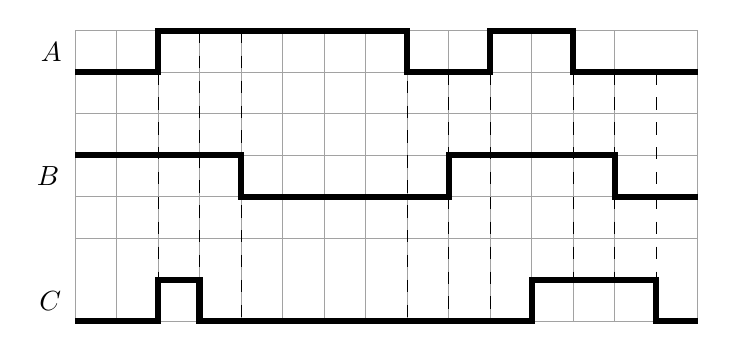
\begin{tikzpicture}[x=0.75pt,y=0.75pt,yscale=-1,xscale=1]
%uncomment if require: \path (0,300); %set diagram left start at 0, and has height of 300

%Shape: Grid [id:dp34531111101152123] 
\draw  [draw opacity=0] (100,40) -- (400,40) -- (400,180) -- (100,180) -- cycle ; \draw  [color={rgb, 255:red, 162; green, 162; blue, 162 }  ,draw opacity=1 ] (120,40) -- (120,180)(140,40) -- (140,180)(160,40) -- (160,180)(180,40) -- (180,180)(200,40) -- (200,180)(220,40) -- (220,180)(240,40) -- (240,180)(260,40) -- (260,180)(280,40) -- (280,180)(300,40) -- (300,180)(320,40) -- (320,180)(340,40) -- (340,180)(360,40) -- (360,180) ; \draw  [color={rgb, 255:red, 162; green, 162; blue, 162 }  ,draw opacity=1 ] (100,60) -- (400,60)(100,80) -- (400,80)(100,100) -- (400,100)(100,120) -- (400,120)(100,140) -- (400,140) ; \draw  [color={rgb, 255:red, 162; green, 162; blue, 162 }  ,draw opacity=1 ] (100,40) -- (400,40) -- (400,180) -- (100,180) -- cycle ;
%Straight Lines [id:da9908667716444586] 
\draw  [dash pattern={on 4.5pt off 4.5pt}]  (140,60) -- (140,160) ;


%Straight Lines [id:da9489034074703155] 
\draw  [dash pattern={on 4.5pt off 4.5pt}]  (160,40) -- (160,160) ;


%Straight Lines [id:da7444148673969375] 
\draw  [dash pattern={on 4.5pt off 4.5pt}]  (180,40) -- (180,180) ;


%Straight Lines [id:da33359589579811755] 
\draw  [dash pattern={on 4.5pt off 4.5pt}]  (260,40) -- (260,180) ;


%Straight Lines [id:da1689198722872045] 
\draw  [dash pattern={on 4.5pt off 4.5pt}]  (280,60) -- (280,180) ;


%Straight Lines [id:da2835936693187402] 
\draw  [dash pattern={on 4.5pt off 4.5pt}]  (300,60) -- (300,180) ;


%Straight Lines [id:da7069604701418795] 
\draw  [dash pattern={on 4.5pt off 4.5pt}]  (340,60) -- (340,160) ;


%Straight Lines [id:da35256438922338873] 
\draw  [dash pattern={on 4.5pt off 4.5pt}]  (360,60) -- (360,160) ;


%Straight Lines [id:da8396949759627998] 
\draw  [dash pattern={on 4.5pt off 4.5pt}]  (380,60) -- (380,160) ;


%Straight Lines [id:da8850959184881091] 
\draw [line width=2.25]    (100,60) -- (140,60) -- (140,40) -- (260,40) -- (260,60) -- (300,60) -- (300,40) -- (340,40) -- (340,60) -- (400,60) ;


%Straight Lines [id:da2574956876601695] 
\draw [line width=2.25]    (100,180) -- (140,180) -- (140,160) -- (160,160) -- (160,180) -- (320,180) -- (320,160) -- (380,160) -- (380,180) -- (400,180) ;


%Straight Lines [id:da8609754683162194] 
\draw [line width=2.25]    (100,100) -- (180,100) -- (180,120) -- (280,120) -- (280,100) -- (360,100) -- (360,120) -- (400,120) ;



% Text Node
\draw (88.5,50) node   {$A$};
% Text Node
\draw (87,110) node   {$B$};
% Text Node
\draw (88,170) node   {$C$};


\end{tikzpicture}
}
\end{frame}


\begin{frame}{Aproximação de Padé}
\begin{block}{Formulação matemática}
\begin{itemize}
    \item O processo de amostragem e o circuito segurador introduzem um \textbf{atraso de tempo} que deve ser compensado para evitar uma possível instabilidade no sistema quando for introduzido o controlador discreto.
\end{itemize}
$$G_{ZOH} = \dfrac{1 - \text{e}^{-sT}}{s}$$
\begin{itemize}
    \item A aproximação de Padé de primeira ordem é dada por:
\end{itemize}
$$\text{e}^{-sT} = \dfrac{1 - \dfrac{sT}{2}}{1+\dfrac{sT}{2}}$$
\end{block}
\end{frame}

\begin{frame}{Aproximação de Padé}
\begin{block}{Formulação matemática}
\begin{itemize}
    \item Deste modo,
\end{itemize}
$$G_h(s)=\dfrac{2}{s+\dfrac{2}{T}}$$
\begin{itemize}
    \item Se observarmos o \textbf{ganho em baixa frequência} dessa função, perceberemos que este é diferente de 1. Porém, o interesse dessa aproximação é determinar uma função que represente apenas o atraso de fase implementado gerado pelo ZOH e que não afete o ganho de malha fechada. Então:
\end{itemize}
$$\boxed{G_h(s)=\dfrac{\dfrac{2}{T}}{s+\dfrac{2}{T}}}$$
\end{block}
\end{frame}

\begin{frame}{Emulação}
\begin{block}{Considerações}
\begin{itemize}
    \item A \textbf{emulação} consiste em projetar um controlador contínuo, prevendo o efeito do ZOH. Após a obtenção do controlador contínuo, basta utilizar uma das aproximações para obter o controlador discreto.
    \item A implementação do controlador discreto se dá por meio de uma \textbf{equação de diferenças}.
    \item O controlador discreto pode ser simulado e testado na malha de controle digital (após a \textbf{discretização da planta via ZOH}) para a verificação dos requisitos de desempenho.
    \item Existem duas técnicas para projetar um controlador digital por emulação:
    \begin{enumerate}
        \item Projeto pelo lugar das raízes;
        \item Projeto pela imposição algébrica de polos.
    \end{enumerate}
\end{itemize}
\end{block}
\end{frame}

\begin{frame}{Projeto pelo lugar das raízes - Exemplo \#01}
\begin{block}{Problema}
	Implementar um controlador discreto por emulação, utilizando o lugar das raízes, para a planta
	$$ G_p(s)=\dfrac{1}{s(s+1)}, $$
	de modo que $ M_p=16,3\% $ e $ T_p=\; $\SI{1}{\second}, quando um degrau for aplicado na entrada.
\end{block}
\end{frame}


\begin{frame}{Projeto pelo lugar das raízes - Exemplo \#01}
\begin{block}{Resolução}
\begin{itemize}
    \item Utilizando as métricas de desempenho que foram dadas:
\end{itemize}
	\begin{align*}
		M_p&=\exp{\left( \dfrac{-\pi\zeta}{\sqrt{1-\zeta^{2}}}\right) }\rightarrow \ln\num{0,163}=\dfrac{-\pi\zeta}{\sqrt{1-\zeta^{2}}}\rightarrow\zeta\approx\num{0,5}\\
		T_p&=\dfrac{\pi}{\omega_d}\therefore 1=\dfrac{\pi}{\omega_d}\rightarrow\omega_d=\pi\;\si{\radian\per\second}\therefore\omega_n=\SI{3,628}{\radian\per\second}
	\end{align*}
\begin{itemize}
    \item Com isso, os polos complexos dominantes devem estar localizados em:
\end{itemize}
	
	\[ s_{1,2}=-\zeta\omega_n\pm j\omega_d\Rightarrow s_{1,2}=-\num{1,81}\pm j\pi \]

\begin{itemize}
    \item A resposta transitória apresenta oscilações com período:
\end{itemize}

	\[ T_d=\dfrac{2\pi}{\omega_d}=\dfrac{2\pi}{\pi}=\SI{2}{\second} \]
\end{block}
\end{frame}


\begin{frame}{Projeto pelo lugar das raízes - Exemplo \#01}
\begin{block}{Resolução}
\begin{itemize}
    \item Escolhe-se um período de amostragem pelo menos $ 10\times $ menor. Logo,
\end{itemize}
	 
	\[ T=\SI{0,2}{\second} \]
	
	\smallskip
	
\begin{itemize}
    \item Sendo assim,
\end{itemize}
	
	\[ G_h(s)=\dfrac{10}{s+10} \]
	
	\begin{itemize}
		\item O próximo passo consiste em escolher uma controlador $ G_c(s) $ de modo que o \textbf{lugar das raízes passe pelos polos desejados} $ s_{1,2} $:
		
		\[ G_c(s)=\dfrac{K(s+z)}{(s+p)} \]
	\end{itemize}
\end{block}
\end{frame}

\begin{frame}{Projeto pelo lugar das raízes - Exemplo \#01}
\begin{block}{Resolução}
\begin{itemize}
    \item O sistema em malha aberta (considerando o controlador contínuo, a aproximação de Padé e a planta) é:
\end{itemize}
	\[\text{sysMA}=\dfrac{K(s+z)}{(s+p)}\cdot\dfrac{10}{s+10}\cdot\dfrac{1}{s(s+1)} \]
\end{block}
\end{frame}

\begin{frame}{Projeto pelo lugar das raízes - Exemplo \#01}
\centerline{
\includegraphics[width=0.8\linewidth]{Figuras/Ch10/fig1.png}}
\end{frame}


\begin{frame}{Projeto pelo lugar das raízes - Exemplo \#01}
\begin{block}{Resolução}
\begin{itemize}
    \item Uma possível solução para encontrar $z$ é cancelar o polo estável da planta com o zero do controlador. Sendo assim, cancelando o polo estável ($ s+1 $) da planta, tem-se que $ z=1 $. Logo,
\end{itemize}
	
	\[ \text{sysMA}=\frac{10K}{(s+p)(s+10)s} \]

\begin{itemize}
    \item Calcula-se $ p $ pela condição de fase:
\end{itemize}

	\begin{align*}
		\left. \left( -\underbrace{ \strut\phase{s}}_{\ang{-60}}-\underbrace{ \strut\phase{s+10}}_{\ang{21}}-\underbrace{ \strut\phase{s+p}}_{\tg^{-1}\frac{\pi}{p-\num{1,81}}}\right)\right| _{s=-\num{1,81}+j\pi}=-180^{\circ}\\
		-219^{\circ}=-\tg^{-1}\left(\dfrac{\pi}{p-\num{1,81}} \right)=-\num{0,80}=\dfrac{-\pi}{p-\num{1,81}}\rightarrow p\approx\num{5,69} 
	\end{align*}
\end{block}
\end{frame}


\begin{frame}{Projeto pelo lugar das raízes - Exemplo \#01}
\begin{block}{Resolução}
\begin{itemize}
    \item Calcula-se $ K $ pela condição de módulo:
\end{itemize}

	\[ \left| sysMA \right|=1 \rightarrow \eval{\left| \dfrac{10K}{(s+\num{5,7})(s+10)s}\right|}_{s=\num{-1.81}+j\pi}=1\Rightarrow K\approx \num{15,88} \]

\begin{itemize}
    \item Com isso, o \textbf{controlador contínuo} é dado por:
\end{itemize}
	
	\[ G_c(s)=\dfrac{\num{15,88}(s+1)}{s+\num{5,69}} \]
\end{block}
\end{frame}

\begin{frame}{Projeto pelo lugar das raízes - Exemplo \#01}
\centerline{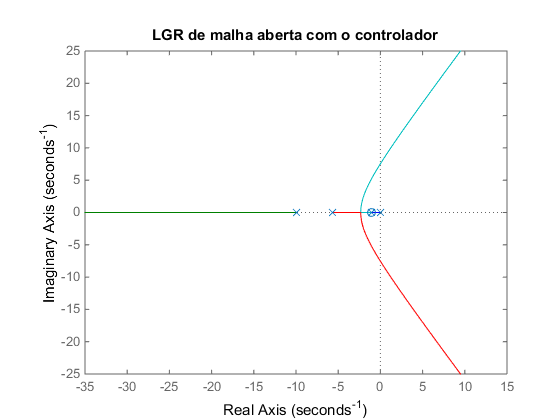
\includegraphics[width=0.8\linewidth]{Figuras/Ch10/fig2.png}}
\end{frame}


\begin{frame}{Projeto pelo lugar das raízes - Exemplo \#01}
\begin{block}{Resolução}
\begin{itemize}
    \item Para obter o \textbf{controlador discreto} podemos utilizar a aproximação do mapeamento polo-zero:
\end{itemize}

	\begin{enumerate}
		\item N/A.
		\item $ G_c(s) $ possui polo em $ s=-\num{5,69} $, logo $ G_c(z) $ possui polo em $z=\num{0,3205} $.
		\item N/A.
		\item $ G_c(s) $ possui zero em $ s=-\num{1} $, logo $ G_c(z) $ possui zero em $z=\num{0,8187} $.
		\item N/A. 
		\[ G_c(z)=\dfrac{K(z-\num{0,8187})}{z-\num{0,3205}} \]
		\item
		\[
		G_c(s)\Big|_{s=0}=G_c(z)\Big|_{z=1}\Rightarrow \dfrac{\num{15,88}}{\num{5,69}}=\dfrac{\num{0,1813}K}{\num{0,6795}}\Rightarrow K=\num{10,46} \]
	\end{enumerate}
\end{block}
\end{frame}

\begin{frame}{Projeto pelo lugar das raízes - Exemplo \#01}
\begin{block}{Resolução}
$$\dfrac{U(z)}{E(z)}=\dfrac{\num{10,46}(z-\num{0,8187})}{z-\num{0,3205}}$$

$$u[k+1] - \num{0,3205} u[k]=\num{10,46}e[k+1]-\num{8,5636}e[k]$$

Aplicando um atraso, temos:\\
$$u[k]=\num{0,3205}u[k-1]+\num{10,46}e[k]-\num{8,5636}e[k-1]$$
\end{block}
\end{frame}

\begin{frame}{Projeto pelo lugar das raízes - Exemplo \#01}
\begin{block}{Resolução}
\begin{itemize}
    \item Para verificar a resposta temporal do sistema discreto, o primeiro passo é \textbf{discretizar a planta via ZOH} (\textit{a cargo do leitor}):
\end{itemize}
$$G_p(z)=(1-z^{-1})\mathcal{Z}\left\lbrace \mathcal{L}^{-1}\eval{\left\lbrace \dfrac{G_p(s)}{s}\right\rbrace}_{t=kT} \right\rbrace =\dfrac{\num{0,0187}(z+\num{0,9355})}{(z-1)(z-\num{0,8187})}$$
\begin{itemize}
    \item A \textbf{função de transferência em malha fechada} é, portanto,
\end{itemize}
$$\dfrac{Y(z)}{R(z)}=\dfrac{G_c(z)G_p(z)}{1+G_c(z)G_p(z)}=\dfrac{\num{0,1959}z+\num{0,1833}}{z^{2}-\num{1,1246}z+\num{0,5038}}$$

$$y[k]=\num{1,1246}y[k-1]-\num{0,5038}y[k-2]+\num{0,1959}r[k-1]+\num{0,1833}r[k-2]$$
\end{block}
\end{frame}

\begin{frame}{Projeto pelo lugar das raízes - Exemplo \#01}
\centerline{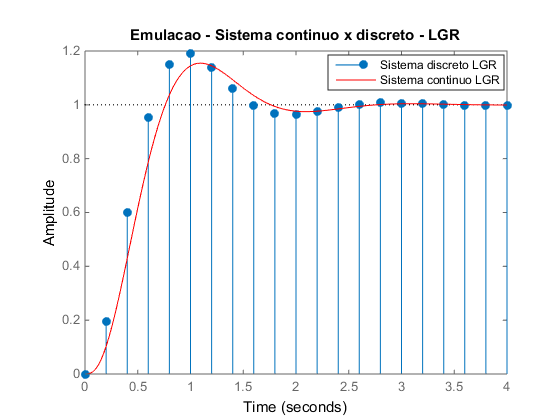
\includegraphics[width=0.8\linewidth]{Figuras/Ch10/fig3.png}}
\end{frame}

\begin{frame}{Projeto pela imposição algébrica de polos - Exemplo \#01}
\begin{block}{Problema}
	Implementar um controlador discreto por emulação, utilizando a imposição algébrica de polos, para a planta
	$$ G_p(s)=\dfrac{1}{s(s+1)}, $$
	de modo que $ M_p=16,3\% $ e $ T_p=\; $\SI{1}{\second}, quando um degrau for aplicado na entrada.
\end{block}
\end{frame}


\begin{frame}{Projeto pela imposição algébrica de polos - Exemplo \#01}
\begin{block}{Resolução}
\begin{itemize}
    \item Nesta técnica \textbf{os polos do controlador são alocados} na posição que atenda às especificações do projeto.
\end{itemize}
	\[ \left. \begin{aligned}
	G_p(s)&=\dfrac{1}{s(s+1)}\\
	G_h(s)&=\dfrac{10}{s+10}
	\end{aligned}\right\rbrace \text{ grau $ n=3 $, o controlador deve ter grau $ m\geqslant n-1 $.} \]
\begin{itemize}
    \item Assume-se $ m=2 $, logo
\end{itemize}
$$ G_c(s)=K\dfrac{(s+z_1)(s+z_2)}{(s+p_1)(s+p_2)} $$
\end{block}
\end{frame}

\begin{frame}{Projeto pela imposição algébrica de polos - Exemplo \#01}
\begin{block}{Resolução}
\begin{itemize}
    \item O sistema em malha aberta (considerando o controlador contínuo, a aproximação de Padé e a planta) é:
\end{itemize}
	\[\text{sysMA}=K\dfrac{(s+z_1)(s+z_2)}{(s+p_1)(s+p_2)}\cdot\dfrac{10}{s+10}\cdot\dfrac{1}{s(s+1)} \]
\end{block}
\end{frame}

\begin{frame}{Projeto pela imposição algébrica de polos - Exemplo \#01}
\centerline{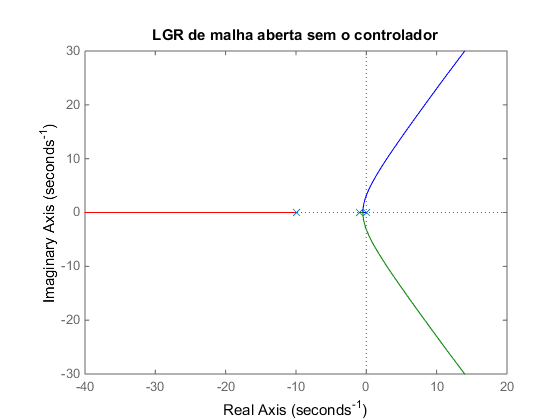
\includegraphics[width=0.8\linewidth]{Figuras/Ch10/fig4.png}}
\end{frame}


\begin{frame}{Projeto pela imposição algébrica de polos - Exemplo \#01}
	\begin{block}{Resolução}
\begin{itemize}
    \item Uma possível solução para encontrar $z_1$ e $z_2$ é cancelar os polos estáveis do sistema em malha aberta com os zeros do controlador. Sendo assim, cancelando o polo estável ($ s+1 $) do sistema em malha aberta, tem-se que $ z_1=1 $. De semelhante modo, cancelando o polo estável ($ s+10 $) do sistema em malha aberta, tem-se que $ z_2=10 $. Logo,
\end{itemize}
	\[ \text{sysMA}=\frac{10K}{(s+p_1)(s+p_2)s} \]
\begin{itemize}
\vspace{-0.2cm}
    \item A \textbf{função de transferência de malha fechada} é dada por:
\end{itemize}		
		\[ \text{sysMF}=\dfrac{10K}{[(s+p_1)(s+p_2)s]+10K} \]
\begin{itemize}
\vspace{-0.2cm}
    \item Deste modo, a equação característica pode ser expressa como sendo:
\end{itemize}
\[  D(s)=s^{3}+(p_1+p_2)s^{2}+p_1p_2s+10K \]
	\end{block}
\end{frame}


\begin{frame}{Projeto pela imposição algébrica de polos - Exemplo \#01}
	\begin{block}{Resolução}
\begin{itemize}
    \item Como a planta é a mesma do exemplo do projeto pelo LGR, sabemos que os polos complexos dominantes devem estar localizados em:
\end{itemize}	
$$s_{1,2}=-\num{1,81}\pm j\pi$$
\begin{itemize}
    \item $D(s)$ é um polinômio de terceira ordem (\textit{slide anterior}); sendo assim, precisamos comparar com outro polinômio de terceira ordem.
    \item \textbf{Obs.:} Para que sistemas de terceira ordem tenham resposta semelhante aos de segunda ordem, deve-se adotar o terceiro polo pelo menos $ \bm{5\times} $ maior que os \textbf{dominantes}.
\end{itemize}	
$$5\zeta\omega_n=\num{9,05}$$
\begin{itemize}
    \item Adota-se $ s_3=-15 $.
\end{itemize}

\end{block}
\end{frame}

\begin{frame}{Projeto pela imposição algébrica de polos - Exemplo \#01}
	\begin{block}{Resolução}
\begin{itemize}
    \item Deste modo, a equação característica pode ser expressa como sendo:
\end{itemize}
		\begin{align*}
			D(s)&=(s+15)(s+\num{1,81}-\num{3,14}j)(s+\num{1,81}+\num{3,14}j)\\
			D(s)&=s^{3}+\num{18,62}s^{2}+\num{67,44}s+\num{197,1}
		\end{align*}
		\vspace{-0.3cm}
\begin{itemize}
    \item Comparando as duas equações características, obtém-se:
\end{itemize}		
		\begin{gather*}
			K=\num{19,7}\\
			p_1=\num{4,92}\\
			p_2=\num{13,7}
		\end{gather*}
		\vspace{-0.3cm}
\begin{itemize}
    \item Com isso, o \textbf{controlador contínuo} é dado por:
\end{itemize}
		\[ G_c(s)=\dfrac{\num{19,7}(s+1)(s+10)}{(s+\num{4,92})(s+\num{13,7})} \]
\end{block}
\end{frame}

\begin{frame}{Projeto pela imposição algébrica de polos - Exemplo \#01}
\centerline{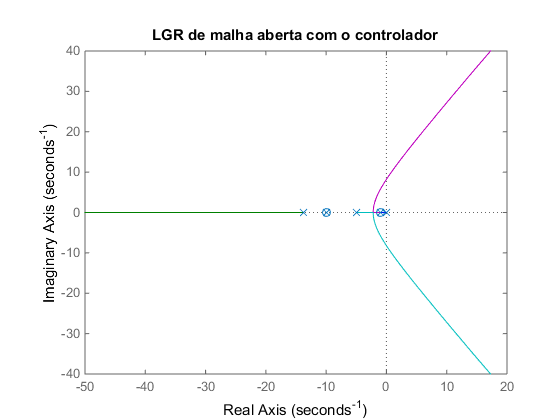
\includegraphics[width=0.8\linewidth]{Figuras/Ch10/fig5.png}}
\end{frame}

\begin{frame}{Projeto pela imposição algébrica de polos - Exemplo \#01}
\begin{block}{Resolução}
\begin{itemize}
    \item Para obter o \textbf{controlador discreto} podemos utilizar a aproximação do mapeamento polo-zero:
\end{itemize}

	\begin{enumerate}
		\item N/A.
		\item $ G_c(s) $ possui polo em $ s=-\num{4,92} $, logo $ G_c(z) $ possui polo em $z=\num{0,37} $.
		$ G_c(s) $ possui polo em $ s=-\num{13,7} $, logo $ G_c(z) $ possui polo em $z=\num{0,064} $.
		\item N/A.
		\item $ G_c(s) $ possui zero em $ s=-\num{1} $, logo $ G_c(z) $ possui zero em $z=\num{0,8187} $.
		$ G_c(s) $ possui zero em $ s=-\num{10} $, logo $ G_c(z) $ possui zero em $z=\num{0,135} $.
		\item N/A. 
		\[ G_c(z)=\dfrac{K(z-\num{0,8187})(z-\num{0,135})}{(z-\num{0,37})(z-\num{0,064})} \]
		\vspace{-0.7cm}
		\item
		\[
		G_c(s)\Big|_{s=0}=G_c(z)\Big|_{z=1}\Rightarrow \dfrac{\num{197}}{\num{67,4}}=\dfrac{\num{0,157}K}{\num{0,589}}\Rightarrow K=\num{10,98} \]
	\end{enumerate}
\end{block}
\end{frame}

\begin{frame}{Projeto pela imposição algébrica de polos - Exemplo \#01}
\begin{block}{Resolução}
$$\dfrac{U(z)}{E(z)}=\dfrac{\num{10,98}(z-\num{0,8187})(z-\num{0,135})}{(z-\num{0,37})(z-\num{0,064})}$$

$$u[k+2] - \num{0,434} u[k+1] + \num{0,0236} u[k] =\num{10,98}e[k+2]-\num{10,471}e[k+1]+\num{1,213}e[k]$$

Aplicando dois atrasos, temos:
$$u[k] = \num{0,434} u[k-1] - \num{0,0236} u[k-2] + \num{10,98}e[k]-\num{10,471}e[k-1]+\num{1,213}e[k-2]$$
\end{block}
\end{frame}

\begin{frame}{Projeto pela imposição algébrica de polos - Exemplo \#01}
\begin{block}{Resolução}
\begin{itemize}
    \item Para verificar a resposta temporal do sistema discreto, o primeiro passo é \textbf{discretizar a planta via ZOH} (\textit{igual ao exemplo anterior}):
\end{itemize}
$$G_p(z)=(1-z^{-1})\mathcal{Z}\left\lbrace \mathcal{L}^{-1}\eval{\left\lbrace \dfrac{G_p(s)}{s}\right\rbrace}_{t=kT} \right\rbrace =\dfrac{\num{0,0187}(z+\num{0,9355})}{(z-1)(z-\num{0,8187})}$$
\begin{itemize}
    \item A \textbf{função de transferência em malha fechada} é, portanto,
\end{itemize}
$$\dfrac{Y(z)}{R(z)}=\dfrac{G_c(z)G_p(z)}{1+G_c(z)G_p(z)}=\dfrac{\num{0,2043}z^3-\num{0,0037}z^2-\num{0,1597}z+\num{0,0211}}{z^{4}-\num{2,053}z^3+\num{1,636}z^2-\num{0,5625}z + \num{0,0409}}$$
\begin{align*}
    y[k]&=\num{2,053}y[k-1]-\num{1,636}y[k-2]+ \num{0,5625}y[k-3]-\num{0,0409}y[k-4] \\
    &+\num{0,2043}r[k-1]-\num{0,0037}r[k-2]-\num{0,1597}r[k-3]+\num{0,0211}r[k-4]
\end{align*}
\end{block}
\end{frame}

\begin{frame}{Projeto pela imposição algébrica de polos - Exemplo \#01}
\centerline{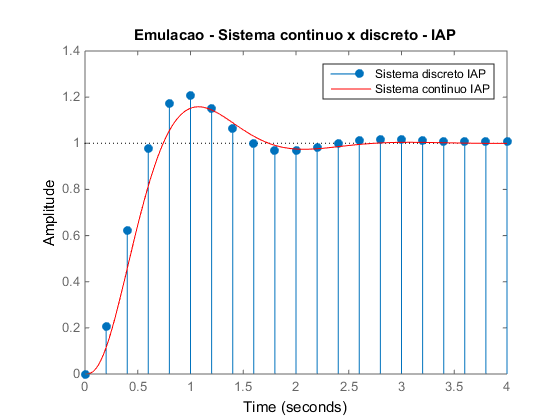
\includegraphics[width=0.8\linewidth]{Figuras/Ch10/fig6.png}}
\end{frame}

\begin{frame}{Comparação entre os métodos}
\centerline{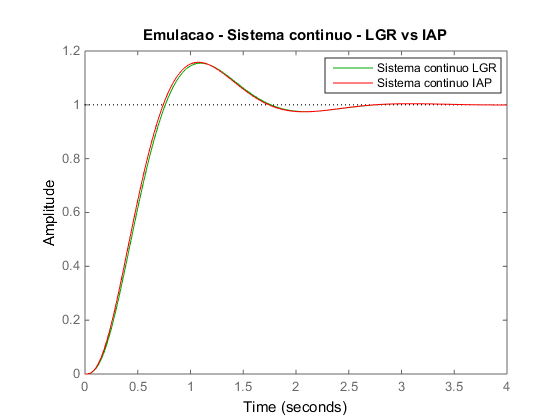
\includegraphics[width=0.8\linewidth]{Figuras/Ch10/fig7.png}}
\end{frame}

\begin{frame}{Comparação entre os métodos}
\centerline{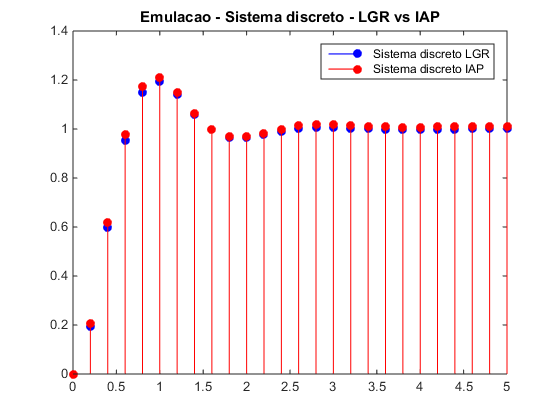
\includegraphics[width=0.8\linewidth]{Figuras/Ch10/fig8.png}}
\end{frame}

\frame{
\frametitle{Exercícios}
\begin{block}{}
01. Considere o diagrama de blocos de um sistema em malha fechada.
\begin{enumerate}
    \item[(a)] Projete um controlador digital, por emulação, utilizando a técnica do lugar das raízes, sabendo que é desejado que os polos dominantes tenham um fator de amortecimento de $\num{0,5}$ e um tempo de acomodação de $2$ s para uma entrada em degrau. Assuma T = $T_d/9$ s. Determine ainda o erro em regime permanente para uma entrada $r(t) = e^2  t$, para todo $t \geq 0$, onde $e$ é uma constante matemática, conhecida como o número de Euler.
    \item[(b)] Repita considerando a técnica da imposição algébrica de polos.
    \item[(c)] Simule e compare os resultados pelo \MATLAB.
\end{enumerate}
\end{block}
\centerline{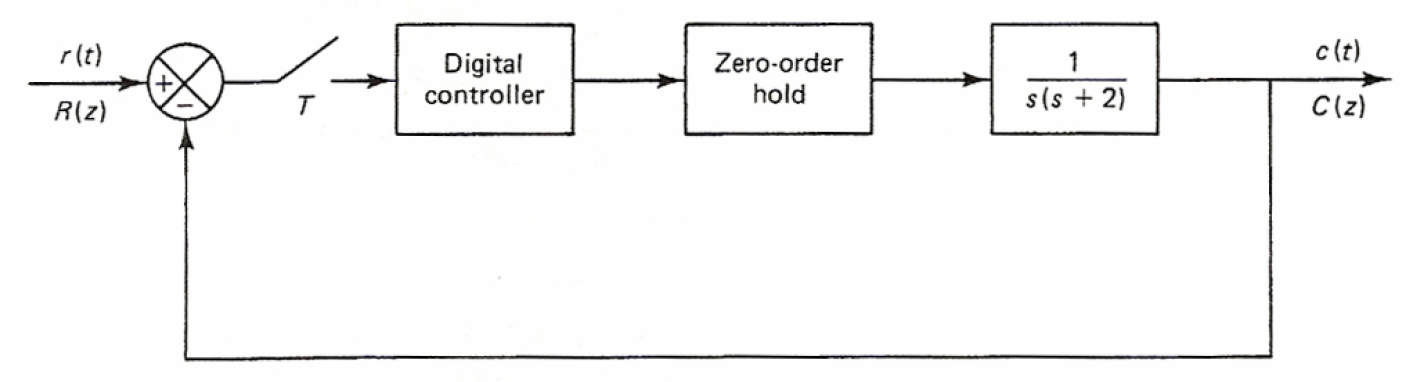
\includegraphics[width=0.85\linewidth]{Figuras/Ch10/fig9.PNG}}
}

\frame{
\frametitle{Referências e exercícios complementares}
\begin{itemize}
\item FRANKLIN, Gene F.; POWELL, J. David; WOLKMAN, Michael L. Digital Control of Dynamic Systems, 3 ed. Addison-Wesley, 1998.
\end{itemize}
\centering{\alert{Página 270 - \textbf{Capítulo 7}}}
}